\documentclass[a4paper,titlepage,twoside,12pt,leqno]{article}

\usepackage[]{fontspec}
\usepackage{xltxtra}
\usepackage[monogreek]{xgreek}

\newcommand{\en}[1]{\setlanguage{american}#1\setlanguage{monogreek}} % Για υφενώσεις στα αγγλικά

\defaultfontfeatures{Mapping=tex-text%, Scale=MatchLowercase}
} 

% Γραμματοσειρά
\setmainfont[Mapping=tex-text]{DejaVu Sans}


\usepackage{longtable} % για έναν μεγάλο πίνακα
\usepackage{graphicx, array, blindtext}

%Για την εντολή \caption* και την αφαίρεση του πίνακας 1:
\usepackage{caption}


\begin{document}

%Για την αφαίρεση της αρίθμησης των σελίδων
\pagestyle{empty}

\begin{table}[ht]
\caption*{\huge{Σύντομες οδηγίες εκκίνησης}}
\centering
\begin{tabular}{*{2}{m{0.48\textwidth}}}
\hline

\begin{center}
\emph{Εισαγωγική οθόνη}\\
\resizebox*{0.5\textwidth}{0.4\textwidth}{
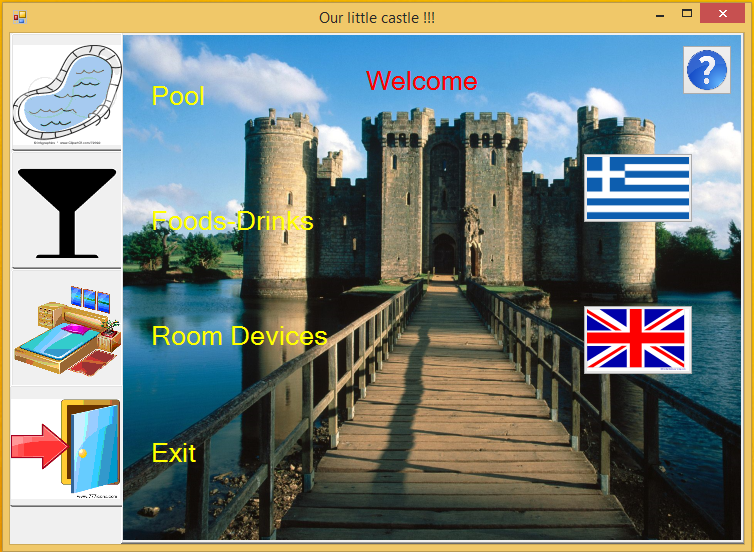
\includegraphics{images/ScreenExit.png}}
\end{center} 

& 
Με την εκκίνηση του προγράμματος ο χρήστης βλέπει την εισαγωγική οθόνη.
Στα αριστερά του παραθύρου φαίνονται τα μενού στα οποία οδηγεί η εφαρμογή ενώ στα δεξιά του παραθύρου φαίνονται σημαίες χωρών και πατώντας σε αυτές αλλάζει η γλώσσα της εφαρμογής. Τα εικονίδια στα αριστερά παραμένουν καθ` όλη την διάρκεια εκτέλεσης της εφαρμογής.\\
\hline

\begin{center}
\emph{Μενού παραγγελίας}\\
\resizebox*{0.5\textwidth}{0.4\textwidth}{
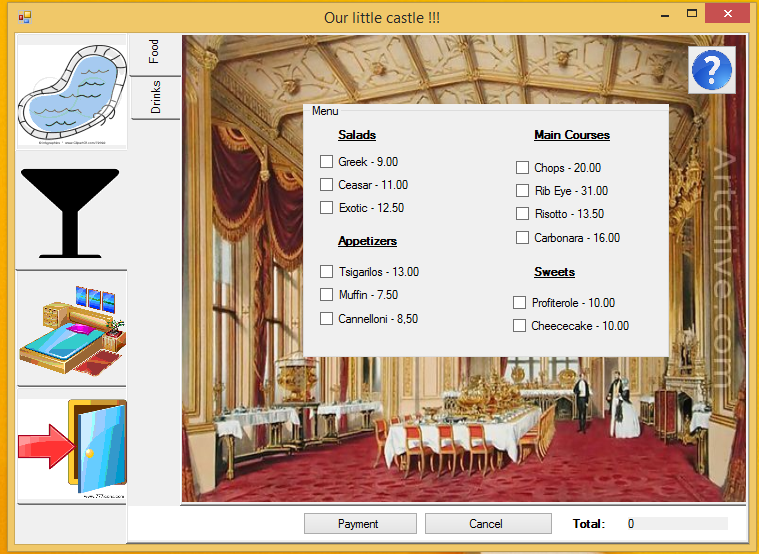
\includegraphics{images/SreenFood.png}}
\end{center} 

& 
Μέσω του μενού παραγγελίας πραγματοποιούνται οι ηλεκτρονικές παραγγελίες. Στα δεξιά της οθόνης φαίνονται τα αντικείμενα που έχει επιλέξει ο χρήστης ενώ μπορεί να γίνει εναλλαγή μεταξύ των φαγητών και των ποτών. \\
\hline

\begin{center}
\emph{Μενού διαχείρισης τάφρου-πισίνας}\\
\resizebox*{0.5\textwidth}{0.4\textwidth}{
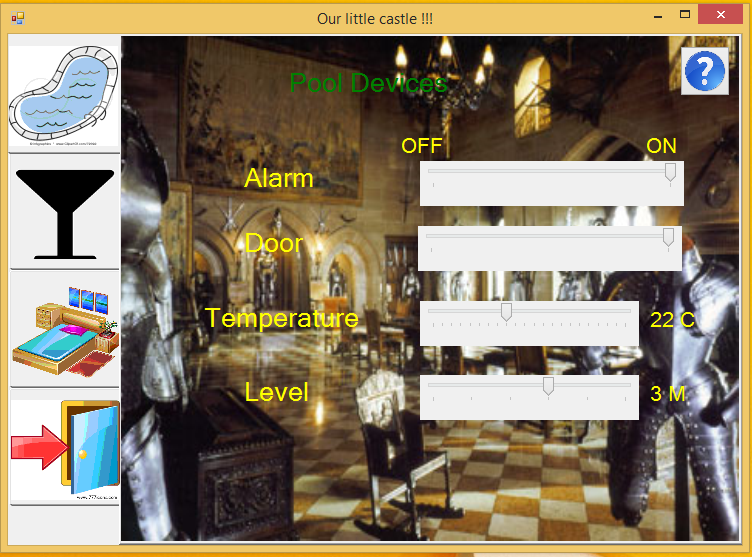
\includegraphics{images/ScreenPool.png}}
\end{center} 

& 
Στο μενού της διαχείρισης της τάφρου-πισίνας ρυθμίζεται η πόρτα της πισίνας, η θερμοκρασία, ο συναγερμός καθώς και η στάθμη της πισίνας μέσω της αντίστοιχης μπάρας. Ο χρήστης μπορεί να προσαρμόσει ότι θέλει για να έχει μία ευχάριστη εμπειρία στην πισίνα. \\
\hline
 
\end{tabular}
\label{table:getting_started}
\end{table}


\begin{table}[ht]
\centering
\begin{tabular}{*{2}{m{0.48\textwidth}}}
\hline


\begin{center}
\emph{Μενού δωματίου}\\
\resizebox*{0.5\textwidth}{0.4\textwidth}{
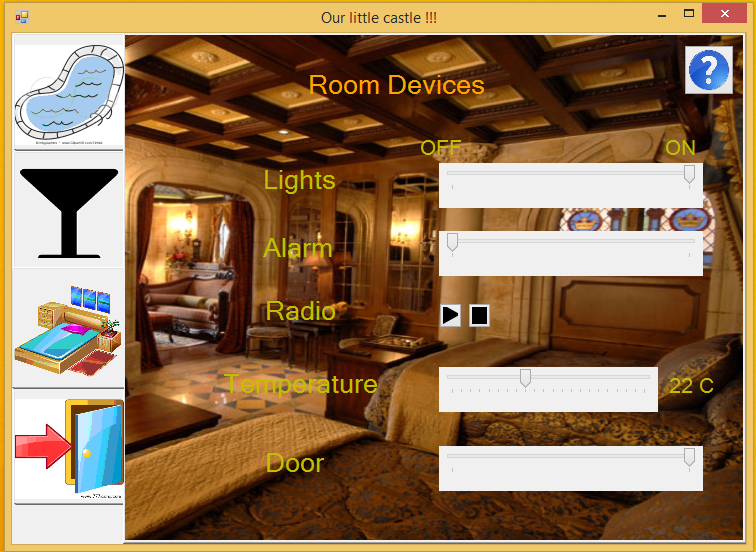
\includegraphics{images/SreenRoom.png}}
\end{center} 

& 
Στο μενού της διαχείρισης των συσκευών του δωματίου ο χρήστης μπορεί να ρυθμίσει κάθε λεπτομέρεια του δωματίου του. Μπορεί να ανοίξει και να κλείσει τα φώτα, το ραδιόφωνο, τον συναγερμό και την πόρτα του δωματίου ενώ μπορεί και να ρυθμίσει την θερμοκρασία του δωματίου και να την φέρει ακριβώς στα μέτρα του.\\
\hline

\end{tabular}
\label{table:getting_started_2}
\end{table}

\end{document}
